\documentclass{article}
\usepackage{graphicx} % Required for inserting images
\usepackage{listings}
\usepackage{xcolor}
\usepackage{float}

\lstset{
  language=C,
  basicstyle=\ttfamily\small,
  keywordstyle=\color{blue}\bfseries,
  commentstyle=\color{gray}\itshape,
  stringstyle=\color{red},
  identifierstyle=\color{black},
  numbers=left,
  numberstyle=\tiny,
  stepnumber=1,
  numbersep=5pt,
  frame=single,
  breaklines=true,
  showstringspaces=false,
  tabsize=2
}

\title{Lab 4 - Parallel algorithms and programming}
\author{ZLATEVSKI Andrej - NEZIRAJ Narta}
\date{April 2026}

\begin{document}

\maketitle

\section{Introduction}

In this report, we explore how to parallelize a fluid simulation using the Lattice Boltzmann Method (LBM) with MPI. The goal is to split the simulation domain across multiple processes and make them communicate efficiently, thus enabling faster computation. Of course, there are limitations, mostly because of the communication overhead between processes and also because of hardware constraints. 

\vspace{5mm}
\textbf{Note:} The CPU used to run the experiments locally is a quad core Intel Core i5-10300H 2.50 GHz with 2 threads per core. With a Grid5000 node in Grenoble, the 2 CPUs are Intel Xeon Gold 6130, 16 cores/CPU.


\section{1D splitting }

The idea of parallelizing the LBM simulation is to split the global domain along the X axis and give each slice to one MPI process. Each process only computes its own part, but needs to exchange boundary values with its neighbors at each time step. We implemented three versions of this communication: a basic blocking version, an odd/even version to avoid processes waiting on each other, and a non blocking version that tries to overlap communication with computation.


\subsection{1D blocking communication}

The core idea of this implementation is to split the domain evenly along the X axis and assign each slice to one MPI process. In lbm\_comm\_init\_ex1(), each process computes its local width as total\_width/comm\_size + 2, where the +2 accounts for the ghost cells on each side. The ghost exchange is done in two phases. In the first phase, each process receives from its left neighbor into its left ghost cell, then sends its last real column to its right neighbor (data propagates from left to right across all ranks). In the second phase, this direction is reversed. Corner cases are handled naturally by the rank checks, for example rank 0 has no left neighbor so it only sends right, and the last rank has no right neighbor so it only sends left. The count is set to comm-$>$height * DIRECTIONS since each column contains one cell per row, and each cell contains 9 directions which are doubles.


\subsection{Limitations}
One limitation of this approach is that blocking communication forces processes to wait on each other, creating a dependency chain where rank 1 waits for rank 0, rank 2 waits for rank 1, and so on. This means communication is done sequentially across all processes, which limits performance (especially when having a large number of processes).

\subsection{1D odd/even communication}
The ghost exchange is done in two phases, one for each direction. In each phase, processes are split into two groups based on their rank, odd ranks send first then receive, while even ranks receive first then send. This avoids the dependency chain from exercise 1 where all processes were waiting on each other, since now half the processes are sending while the other half are receiving simultaneously. Corner cases are handled the same way as before, rank 0 has no left neighbor and the last rank has no right neighbor, so the corresponding send and receive calls are simply skipped.

\subsection{Limitations}
One limitation of this approach is that even though the odd/even pattern avoids the dependency chain, it still uses blocking communication (with SEND/RECV) meaning that each process still has to fully wait for its communication to complete before moving on to the next computation step. This means there is still \textbf{no overlap} between communication and computation.


\subsection{1D non-blocking communication}

To make use of non-blocking communication, we modified the computation step. After applying special cells and collision, we start the ghost exchange with non-blocking calls, then immediately compute the interior cells, the ones that do not depend on ghost cell values. Then we wait for the ghost exchange to finish before computing the border cells that need the received values. This way, communication and computation overlap as much as possible.

All sends and receives are posted at once, and the number of active requests is tracked in comm-$>$req\_count. The key difference is that communication is split into two parts, a start function that posts all the requests, and a wait function that calls MPI\_Waitall. This allows the interior cells to be computed while the ghost exchange is still in progress, overlapping communication with computation and reducing the total execution time.

\subsection{Limitations}
One limitation of this approach is that the overlap between communication and computation can be observed if the interior computation takes long enough to hide the communication latency. For small  sizes, the communication finishes before the interior computation does, meaning the wait call returns immediately and the overlap brings no benefit.

\section{2D splitting}

The core idea of 2D splitting is to divide the global domain into a grid of rectangular sub-domains along both the X and Y axes, rather than simple vertical slices. This approach is more scalable as it reduces the amount of data exchanged relative to the computation (by having less ghost cells). Each process manages a local mesh and must synchronize its boundaries with up to eight neighbors: four direct neighbors (top, bottom, left, right) and four diagonal corner neighbors. By using a 2D grid, the communication overhead is better distributed, especially in simulations with a large number of processes where 1D splitting would result in extremely thin and inefficient domains.

\subsection{2D blocking communication using manual copy of rows}

The implementation in lbm\_comm\_init\_ex4() leverages MPI Cartesian topology through MPI\_Dims\_create() and MPI\_Cart\_create() to automatically handle process placement and coordinate mapping within the 2D grid. The ghost cell exchange in lbm\_comm\_ghost\_exchange\_ex4() is performed in two sequential phases using MPI\_Sendrecv() to minimize the number of communication calls. Since the memory layout stores cells column-wise (contiguous in Y), horizontal exchanges are performed directly on the mesh columns. For vertical exchanges, the non-contiguous row data is manually gathered into buffers before transmission and scattered back after reception. Crucially, by performing the horizontal exchange first and including the updated ghost columns in the subsequent vertical transfer, the implementation correctly propagates corner values to all eight neighbors using only four communication steps, avoiding the need for separate diagonal exchanges. Figure 1 demonstrates this procedure visually: 

\begin{figure}[H]
    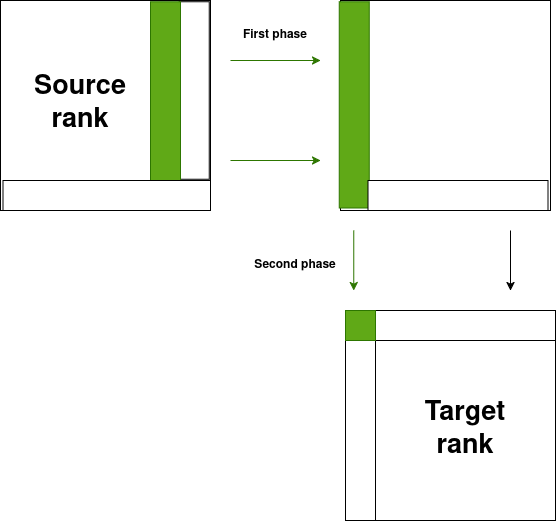
\includegraphics[width=1\linewidth]{corner_exchange.drawio.png}
    \caption{Diagonal values sent in 2 phases}
\end{figure}

\subsection{Limitations}
No matter how good the division of the local mesh is done, whenever a blocking communication is used, it is not a good idea, and the reasons are the same as described above, when 1D splitting is used. 

\subsection{2D blocking communication using MPI Datatypes}

The core idea is the same as exercise 4, but instead of manually copying non contiguous rows into buffers, we create a custom MPI type using MPI\_Type\_vector that expresses a row of the mesh, since rows are not stored next to each other in memory. This type is stored in comm-$>$type and used directly in the communication calls, removing the need for temporary buffers. 

The ghost exchange follows the same direction as exercise 4 using MPI\_Sendrecv. Left and right communications are unchanged since columns are already contiguous in memory. For the top and bottom communications, instead of copying rows into a buffer, we directly pass the starting row address, and with the custom type MPI handles the non contiguous memory access by itself (internally).
\subsection{Limitations}
Here too we have blocking communication. The use of MPI types simplifies the code and avoids the overhead of manual copies, but does not improve the communication pattern itself.
\subsection{2D with non-blocking communication}

The core idea is the same as exercise 5, but using non blocking communication. The ghost exchange is split into two parts (in this way corner cells can't be sent twice). The first part handles the 4 direct neighbors (left, right, up, down) using MPI\_Irecv and MPI\_Isend, then waits for all of them to finish. The second part handles the 4 diagonal neighbors (corners), then waits. Splitting into two parts is necessary because the corner ghost cells could be overwritten or have erroneous data if both batches are dealt at the same time (since the left, right, up or down communication already fill the corner ghost cells when transferring the full border columns and rows).

\subsection{Limitations}
The main limitation is that even though we use non blocking calls, we still wait after each part before starting the next one. This means that there is a slight dependency and the overlapping potential is reduced, however in the second phase, only the corner values are exchanged (4 arrays of doubles), which signifies lower bandwidth, so the overhead of this phase could be neglected (but still it is something to consider). 

\section{Scalability measurements}
After the implementation and testing phase of our work, we decided to run scalability measurements. These measurements are done using a Grid5000 node and a basic laptop. We will compare execution times and efficiency, using strong and weak scaling approaches, as described in class. In the legend, linear split signifies exercise 1 code, i.e blocking 1D splitting communication, and overlap async signifies exercise 6 code, asynchronous 2D splitting communication.
\subsection{Execution times}
\subsubsection{Strong scaling}
Figures 2 and 3 show execution times, using the strong scaling approach. The obvious benefits of splitting the computation are demonstrated. One thing to notice is that linear splitting is less effective than the other types of communication, because of dependencies and processors being idle. Also, the effects of Amdahl's law are visually present, as adding 8 more processes (or cores) do not reduce execution times. Overlapping communication and computation is the most effective approach, and can be seen more clearly in Figure 3. 

\begin{figure}[H]
    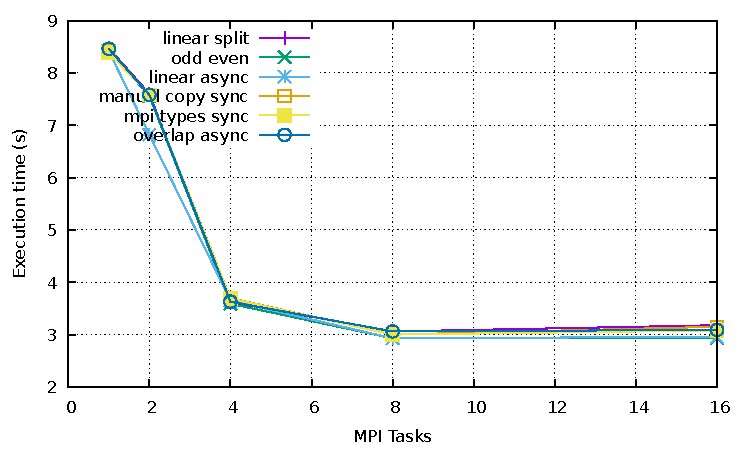
\includegraphics[width=1\linewidth]{scale.pdf}
    \caption{Strong scaling execution times in a Grid5000 compute node}
\end{figure} 

\begin{figure}[H]
    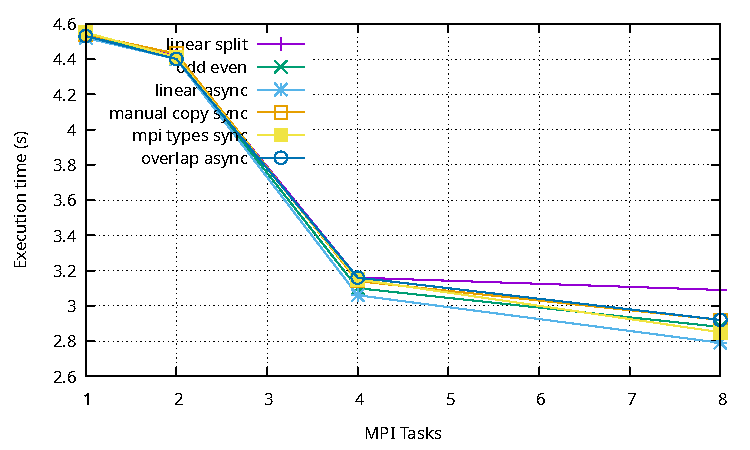
\includegraphics[width=1\linewidth]{scale_strong_local.pdf}
    \caption{Strong scaling execution times in a local machine (laptop)}
\end{figure} 

\subsubsection{Weak scaling}

In weak scaling, the problem size grows linearly with the number of processors. In our case, the mesh gets bigger, not only suggesting a far larger computation time in a rank, but also increasing the bandwidth, which are 2 indicators of slower execution times. The latency stays the same, as each boundary layer is sent only once. What is interesting is displayed in Figure 4: There is a huge spike when the number of MPI processes is 2. And this is not a one time outsider value - we have run multiple times the script for computing the graphs, and the result is always the same. However, we don't have a clear explanation for its occurrence. One thing to note here is the fact that if 1D linear blocking communication is used, the execution time gets far worse, compared to the other approaches, because the computation time in a rank is increased, suggesting even bigger idle processor times!  

\begin{figure}[H]
    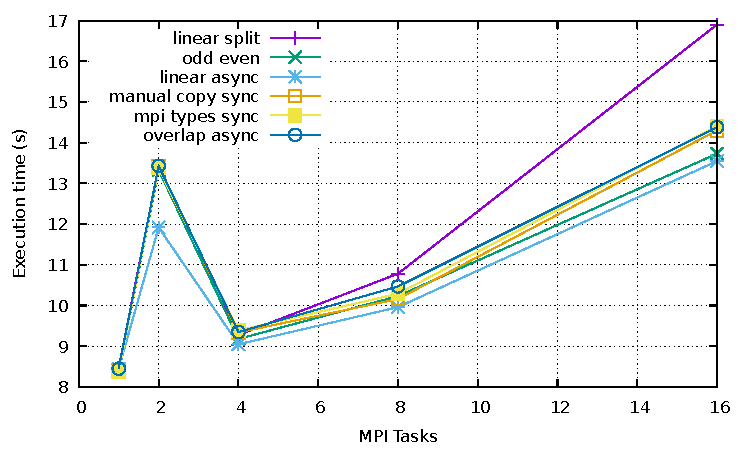
\includegraphics[width=1\linewidth]{scale_weak.pdf}
    \caption{Weak scaling execution times in a Grid5000 compute node}
\end{figure} 

\begin{figure}[H]
    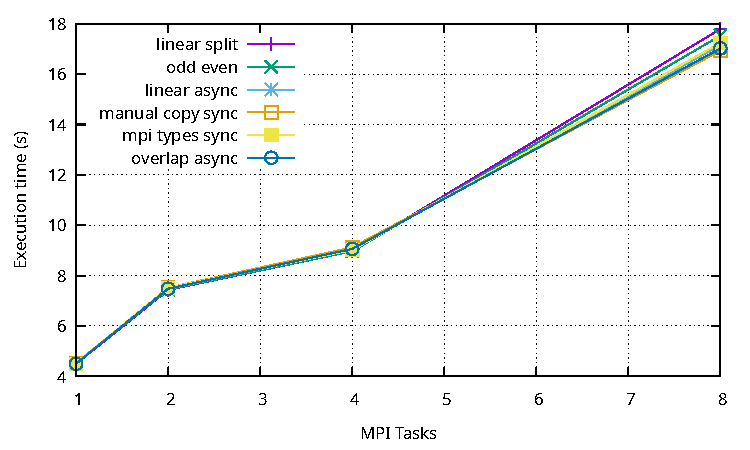
\includegraphics[width=1\linewidth]{scale_weak_local.pdf}
    \caption{Weak scaling execution times in a local machine (laptop)}
\end{figure}

\subsection{Efficiency}
The efficiency of an algorithm is calculated as $E(p) = \frac{T(s)}{p \cdot T(p)}$ where $T(s)$ is time elapsed when the algorithm is run sequentially and $T(p)$ when it is run using $p$ processors. In the following sections, we interpret the results, when using as seen previously, either the strong scaling or weak scaling approach. We do not display results coming from computations done locally, as they are similar, thus boring. Based on the results we obtained previously concerning the execution times, these graphs do make sense. In a more formal way, we could say that this efficiency reduction is due to the fact that we introduce more communication overhead with the number of processes increasing, which is non-existent in the case of 1 process. On top of that, if we are using weak scaling, there is additional computational overhead. 
\subsubsection{Strong scaling}

\begin{figure}[H]
    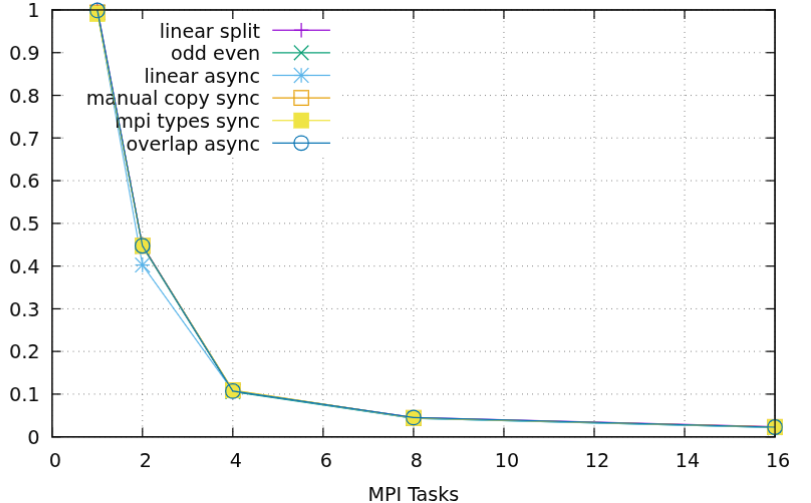
\includegraphics[width=1\linewidth]{efficiency_strong_correct.png}
    \caption{Efficiency calculation during strong scaling}
\end{figure}

\subsubsection{Weak scaling}

\begin{figure}[H]
    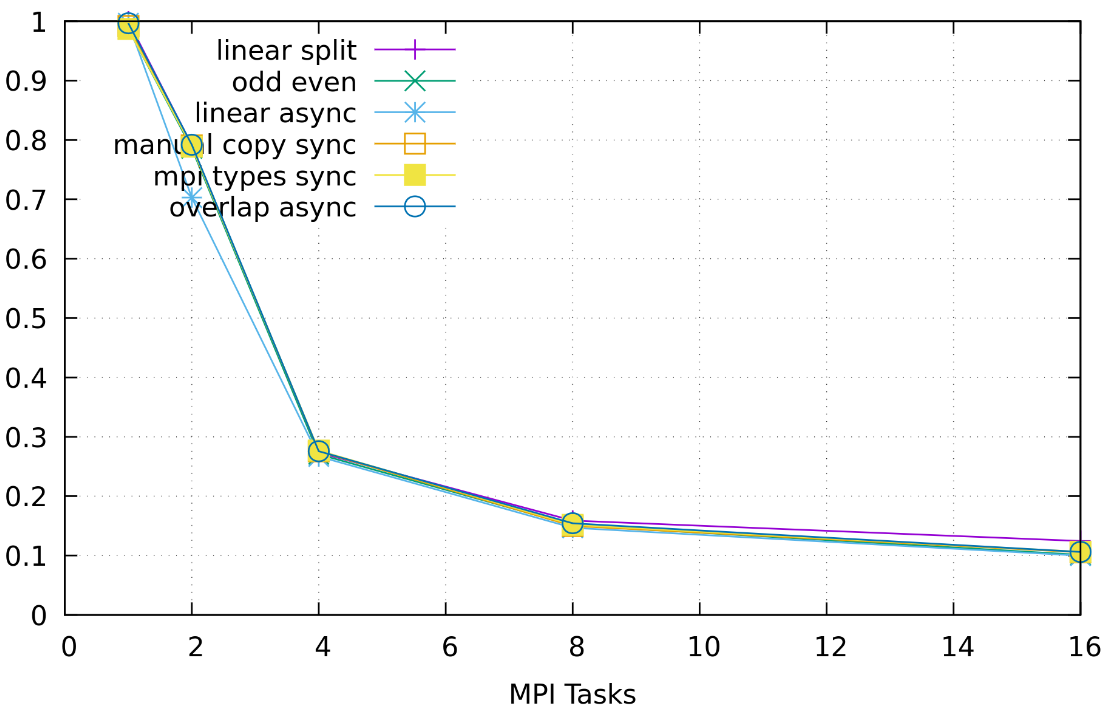
\includegraphics[width=1\linewidth]{efficiency_weak_img.png}
    \caption{Efficiency calculation during weak scaling}
\end{figure}

\section{Conclusion}

In this report, we implemented three variants of 1D domain splitting and three variants of 2D domain splitting for a parallel LBM fluid simulation using MPI. Each variant improved on the previous one,from a simple blocking approach that created a dependency chain between processes, to an odd/even pattern that allowed some parallelism in communication, and finally a non blocking version that overlapped communication with computation. 

The scalability measurements confirm these observations. Strong scaling shows clear execution time improvements as the number of processes increases, with the 2D non blocking version consistently outperforming the 1D blocking one. Weak scaling results show that 1D blocking communication scales badly compared to the other approaches, as the idle processor time grows with the problem size. The efficiency results also confirm that communication and computation overhead increase with the number of processes, which is expected, with the fact that the mesh in question gets bigger each time we add a process.

\end{document}